\section{Introduction and main results}



In this paper, we will consider clustering in a model of random graphs that involves points taken randomly in the hyperbolic plane. This model was introduced by Krioukov, Papadopoulos, Kitsak, Vahdat and Bogu\~{n}\'a~\cite{krioukov2010hyperbolic} in 
2010 - we abbreviate it as \emph{the KPKVB model}. We should however note that the model also goes by several other names in the literature, including {\em hyperbolic random geometric graphs} and {\em random hyperbolic graphs}. Krioukov et al.~suggested this model as a suitable model for complex networks. It exhibits the three main characteristics usually associated with complex networks: a power-law degree distribution, a non-vanishing clustering coefficient and short graph distances.

%
%\subsection{Hyperbolic random graphs}\label{ssec:hyperbolic_model}


We start with the definition of the KPKVB model. As mentioned, its nodes are situated in the hyperbolic plane $\Haa$, which is a surface with constant Gaussian curvature $-1$. This surface has several convenient representations (i.e.~coordinate maps), including the Poincar\'e halfplane model, the Poincar\'e disk model and the Klein disk model. A gentle introduction to Gaussian curvature, hyperbolic geometry and these representations of the hyperbolic plane can be found in~\cite{stillwell2012geometry}. Throughout this paper we will be working with a representation of the hyperbolic plane using {\em hyperbolic polar coordinates}, sometimes called the {\em native representation}. That is, a point $u \in \Haa$ is represented as $(r,\theta)$, where $r$ is the hyperbolic distance between $u$ and the origin $O$ and $\theta$ as the angle between the line segment $Ou$ and the positive $x$-axis. 
Here, when mentioning ``the origin'' and the angle between the line segment and the positive $x$-axis, we think of $\Haa$ embedded as the Poincar\'e disk in the ordinary euclidean plane.

The KPKVB model has three parameters: the number of vertices $n$, which we think of as going to infinity, and $\alpha > \frac{1}{2}$, $\nu > 0$ which we think of as fixed. Given $n, \alpha, \nu$ we define $R = 2\log(n/\nu)$. Then the hyperbolic random graph $G(n;\alpha, \nu)$ is defined as follows:
\begin{itemize}
\item The vertex set is given by $n$ i.i.d.~points $u_1, \dots, u_n$ denoted in polar coordinates $(r_i, \theta_i)$, where the angular coordinate $\theta$ is chosen uniformly from $(-\pi,\pi]$ while the radial coordinate $r$ is sampled independently according to the cumulative distribution function
\begin{equation}\label{eq:def_hyperbolic_point_distribution}
	F_{\alpha,R}(r) = \begin{cases}
		0 &\mbox{if } r < 0\\
		\frac{\cosh(\alpha r)-1}{\cosh(\alpha R) - 1} &\mbox{if } 0 \le r \le R\\
		1&\mbox{if } r > R
	\end{cases}
\end{equation}
\item Any two vertices $u_i=(r_i,\theta_i)$ and $u_j=(r_j,\theta_j)$ are adjacent if and only if $d_\H(u_i,u_j) \le R$, where $d_\H$ denotes the distance in the hyperbolic plane. We will frequently be using that, by the hyperbolic law of cosines, $d_\H(u_i,u_j) \le R$ is equivalent to
\[
	\cosh(r_i) \cosh(r_j) - \sinh(r_i) \sinh( r_j) \cos(|\theta_i-\theta_j|_{2\pi}) \le \cosh(R),
\]
where $|a|_{b} = \min( |a|, b - |a|)$ for $-b\leq a\leq b$.
\end{itemize}

\begin{figure}[!t]
\centering
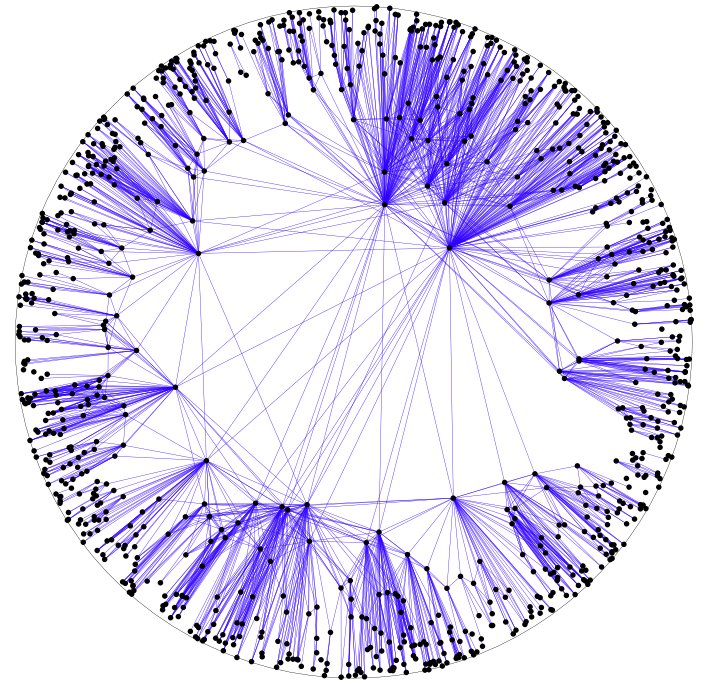
\includegraphics[scale=0.3]{figures/KPKVB.png}
\caption{Simulation $G(n;\alpha, \nu)$ with $\alpha = 0.9$, $\nu = 0.2$ and $n = 5000$.
%\PvdH{@Tobias: this figure (HyperRGG\_N5000L5.eps) is taken from the figures you send me. Could you fill in the value of $\alpha$ and $\nu$ you used for the simulation.}
}
\label{fig:H_graph_example}
\end{figure}

\noindent
Figure~\ref{fig:H_graph_example} shows a computer simulation of $G(n;\alpha, \nu)$.


As observed by Krioukov et al.~\cite{krioukov2010hyperbolic}, and proved rigorously by Gugelmann et al.~\cite{gugelmann2012random}, the degree sequence of the KPKVB model follows a power-law with exponent $2\alpha+1$.
% More specifically, if $N_k$ denotes the number of vertices of degree exactly $k$ then Gugelmann et al.~\cite{gugelmann2012random} have shown that
% 
% \begin{equation}\label{eq:gugeldegseq} 
% N_k = (1+o(1)) \cdot n \cdot p_k \quad \text{ a.a.s., }
% \end{equation}
% 
% \noindent
% where $p_k := 2\alpha \cdot \xi^{2\alpha} \cdot \Gamma^+\left(k - 2\alpha, \xi\right) / k!$
% with, here and in the rest of the paper, $\xi := \frac{4\alpha\nu}{\pi(2\alpha-1)}$ and 
% $\Gamma^+(a,b) := \int_b^\infty t^{a-1} e^{-t} \text{d}t$ the 
% {\em upper incomplete gamma function} and, for $(E_n)_n$ a sequence of events, 
% $E_n$ {\em asymptotically almost surely} (a.a.s.) means that $\Pee(E_n)\to 1$.
%%In particular $X_n = (1+o(1)) Y_n$ is equivalent to $X_n/Y_n \plim 1$.
%In fact~\eqref{eq:gugeldegseq} was shown in~\cite{gugelmann2012random} to hold not only when $k$ is constant but 
%also if $k$ depends on $n$ as long as $k = o( n^\delta )$ for a suitable small constant $\delta = \delta( \alpha )$.
%Standard asymptotic manipulations show that 
%
%$$p_k \sim 2\alpha\xi^{2\alpha} k^{-(2\alpha+1)}, $$
%
%as $k\to\infty$.
%\TM{ \RD{We need to add something like the following} : 
%In Appendix~\ref{} we settle the minor technical point of showing that~\eqref{eq:gugeldegseq} in fact extends 
%to all $k$ with $k \ll n^{1/(2\alpha+1)}$, while 
%$N_k = 0$ a.a.s.~whenever $k \gg n^{1/(2\alpha+1)}$. }
Gugelmann et al.~\cite{gugelmann2012random} also showed that the average degree converges in probability to the constant $8\nu\alpha^2/ \pi (2\alpha-1)^2$, and they showed that the (local) clustering coefficient is non-vanishing in the sense that it is bounded below by a positive constant a.a.s. Here, and in the rest of the paper, for a sequence $(E_n)_n$ of events, $E_n$ {\em asymptotically almost surely} (a.a.s.) means that $\Pee(E_n)\to 1$ as $n \to \infty$.
%Their work however left open the question of whether the clustering coefficient actually converges in probability.

Apart from the degree sequence and clustering, the third main characteristic associated with complex networks, ``short distances'', has also been established in the literature. In~\cite{abdullah2017typical} it is shown that for $\alpha < 1$ the largest component is what is called an \emph{ultra-small world}: if we randomly sample two vertices of the graph then, a.a.s., conditional on them being in the same component, their graph distance is of order $\log\log n$. In~\cite{kiwi2015bound} and~\cite{friedrich2018diameter} a.a.s.~polylogarithmic upper and lower bounds on the graph diameter of the largest component are shown, and in~\cite{muller2017diameter}, these were sharpened to show that $\log n$ is the correct order of the diameter.

Earlier work of the first and third authors with Bode~\cite{bode2015largest} and of the first and third authors~\cite{fountoulakis2018law} has established the ``threshold for a giant component'': if $\alpha < 1$ then there is a unique component of size linear in $n$ no matter how small $\nu$ (i.e. the average degree); if $\alpha > 1$ all components are sublinear no matter the value of $\nu$; and if $\alpha=1$ then there is a critical value $\nu_{\text{c}}$ such that for $\nu < \nu_{\text{c}}$ all components are sublinear and for $\nu > \nu_{\text{c}}$ there is a unique linearly sized component (all of these statements holding a.a.s.). Whether or not there is a giant component if $\alpha=1$ and $\nu=\nu_{\text{c}}$ remains an open problem. In~\cite{kiwi2015bound} and~\cite{kiwi2017second}, Kiwi and Mitsche considered the size of the second largest component and showed that for $\alpha \in (1/2, 1)$, a.a.s., the second largest component has polylogarithmic order with exponent $1/(\alpha -1/2)$.


In another paper of the first and third authors with Bode~\cite{bode2016probability} it was shown that $\alpha=1/2$ is the threshold for connectivity: for $\alpha < 1/2$ the graph is a.a.s.~connected, for $\alpha>1/2$ the graph is a.a.s.~disconnected and when $\alpha=1/2$ the probability of being connected tends to a continuous, nondecreasing function of $\nu$ which is identically one for $\nu \geq \pi$ and strictly less than one for $\nu < \pi$. Friedrich and Krohmer~\cite{blasius2018cliques} studied the size of the largest clique as well as the number of cliques of a given size. Bogu\~{n}a et al.~\cite{boguna2010sustaining} and Bl\"asius et al.~\cite{BlasiusMLE} considered fitting the KPKVB model to data using maximum likelihood estimation. Kiwi and Mitsche~\cite{kiwi2018spectral} studied the spectral gap and related properties, and Bl\"asius et al.\cite{blasius2016hyperbolic} considered the tree-width and related parameters of the KPKVB model. Recently Owada and Yogeshwaran~\cite{owada2018sub} considered subgraph counts, and in particular established a central limit theorem for the number of copies of a fixed tree $T$ in $G(n;\alpha,\nu)$, subject to some restrictions on the parameter $\alpha$.

\subsubsection*{Clustering}

In this work we study the clustering coefficient in the KPKVB model. In the literature there are unfortunately two distinct, rival definitions of the {\em clustering coefficient}. One of those, sometimes called the {\em global} clustering coefficient, is defined as three times the ratio of the number of triangles to the number of paths of length two in the graph. Results for this version of the clustering coefficient in the KPKVB model were obtained by Candellero and the first author~\cite{candellero2016clustering} and for the evolution of graphs on more general spaces with negative curvature by the first author in~\cite{fountoulakis2012evolution}. 

We will study the other notion of clustering, the one which is also considered by Krioukov et al.~\cite{krioukov2010hyperbolic} and Gugelmann et al.~\cite{gugelmann2012random}. It is sometimes called the {\em local} clustering coefficient, although we should point out that Gugelmann et al.~actually call it the global clustering coefficient in their paper. For a graph $G$ and a vertex $v\in V(G)$ we define the clustering coefficient {\em of $v$} as:
\[
	c(v) := \left\{\begin{array}{cl}
		\displaystyle \frac{1}{{\text{deg}(v)\choose 2}} \sum_{u,w\sim v} 1_{\{uw \in E(G)\}}, 
			& \text{ if $\text{deg}(v) \geq 2$, }\\
		& \\
        0, & \text{ otherwise,}
        \end{array}\right.
\]
where $E(G)$ denotes the edge set of $G$ and $\text{deg}(v)$ is the degree of vertex $v$. That is, provided $v$ has degree at least two, $c(v)$ equals the number of edges that are actually present between the neighbours \PvdH{I think it is neighbors in US English vs neighbours in UK English. Is there any specific reason to us the UK version?} of $v$ divided by the number of edges that could possibly be present between the neighbours given the degree of $v$.
The clustering coefficient of $G$ is now defined as the average of $c(v)$ over all vertices $v$:
\[
	c(G) := \frac{1}{|V(G)|} \sum_{v\in V(G)} c(v).
\]

As mentioned above, Gugelmann et al.~\cite{gugelmann2012random}, have established that $c(G(n;\alpha,\nu))$ is non-vanishing a.a.s., but they left open the question of convergence. Theorem~\ref{thm:maincc} below establishes that the clustering coefficient indeed converges in probability to a constant $\gamma$ that we give explicitly as a closed form expression involving $\alpha,\nu$ and several classical special functions.

In addition to the clustering coefficient, we shall also be interested in the {\em clustering function}.
This assigns to each integer $k$ the value
\begin{equation}\label{eq:def_clustering_function}
	c(k; G) := \begin{cases}
		\displaystyle \frac{1}{N_k} \sum_{v \in V(G), \atop \text{deg}(v)=k}  c(v),  &\mbox{ if } N_k \ge 1,\\
		0, &\mbox{else,}
	\end{cases}
\end{equation}
where $N_k$ denotes the number of vertices of degree exactly $k$ in $G$. In other words, the clustering function assigns to the integer $k$ the average of the local clustering coefficient over all vertices of degree $k$. We remark that, while it might seem natural to consider $c(k)$ to be ``undefined'' when $N_k=0$, we prefer to use the above definition for technical 
convenience.  This way $c(k; G(n;\alpha,\nu) )$ is a plain vanilla random variable and we can for instance compute its moments without any issues.

A general expression of the clustering function for KPKVB random graphs is given in~\cite[Equation (59)]{krioukov2010hyperbolic}. The authors conjecture that as $k$ tends to infinity, the clustering function decays as $k^{-1}$. They based this prediction on observations (Figure 8 in \cite{krioukov2010hyperbolic}) in experiments on the infrastructure of the Internet obtained in~\cite{claffy2009internet}. Despite these interesting observations and the attention the KPKVB model has generated since then, the behaviour of the clustering function in KPKVB random graphs had not been completely determined. In particular it has not been established whether it converges as $n\to\infty$ to some suitable limit function, nor how $c(k;G)$ scales with $k$. Theorems~\ref{thm:mainkfixed},~\ref{thm:mainktoinfty} and Proposition~\ref{prop:asymp} below settle these questions. Theorem~\ref{thm:mainkfixed} shows that for each fixed $k$, the value $c(k;G(n;\alpha,\nu))$ converges in probability to a constant $\gamma(k)$ that we again give explicitly as a closed form expression involving $\alpha,\nu$ and several classical special functions. Theorem~\ref{thm:mainktoinfty} extends this result to growing sequences satisfying $k \ll n^{1/(2\alpha+1)}$. Proposition~\ref{prop:asymp} clarifies the asymptotic behavior of the limiting function $\gamma(k)$, as $k\to\infty$. This depends on the parameter $\alpha$, and $\gamma(k)$ only scales with $k^{-1}$ when $\alpha > 3/4$, which corresponds to the exponent of the degree distribution exceeding $5/2$. 
So in particular our findings disprove the abovementioned conjecture of Krioukov et al.~\cite{krioukov2010hyperbolic}.


\subsubsection*{Notation}

In the statement of our main results, and throughout the rest of the paper, we will use the following notations. 
We set 
$$\xi := \frac{4\alpha\nu}{\pi(2\alpha-1)}. $$

We write $\Gamma(z) := \int_0^\infty t^{z-1} e^{-t}\text{d}t$ for the gamma function, 
$\Gamma^+(a,b) := \int_b^\infty t^{a-1} e^{-t}\text{d}t$ for the upper incomplete gamma function, 
 $B(a,b) := \int_0^1 u^{a-1}(1-u)^{b-1}\text{d}u = \Gamma(a)\Gamma(b) / \Gamma(a+b)$ for the beta function and 
 $B^-(x,a,b) := \int_0^x u^{a-1}(1-u)^{b-1}\text{d}u$ for the lower incomplete beta function. 
We write $U(a,b,z)$ for the hypergeometric U-function (also called Tricomi's confluent hypergeometric function), which 
%for $a,b,z\in \mathbb{C}$, $b \not \in \mathbb{Z}_{\leq 0}$, $\mathrm{Re}(a), \mathrm{Re}(z) >0$ 
has the integral representation 
\[
	U(a,b,z) = \frac{1}{\Gamma(a)} \int_0^\infty e^{-zt} t^{a-1} (1+t)^{b-a-1} dt,
\] 
see~\cite[p.255 Equation (2)]{erdelyi1953higher}, and let $\MeijerGnew{m}{\ell}{p}{q}{{\bf a}}{{\bf b}}{z}$ denote 
Meijer's G-Function~\cite{meijer1946gfunction}, see Appendix~\ref{sec:Meijer_G_functions} for more details.

For a sequence $(X_n)_n$ of random variables, we write $X_n \xrightarrow[n\to\infty]{\Pee} X$ to denote that $X_n$ converges in probability to $X$, as $n \to \infty$.

%We further adopt standard notations on asymptotic behavior of functions and sequences. That is, for two functions $f$ and $g$, we write $f(n) = \smallO{g(n)}$ as $n \to \infty$ if $\limsup_{n \to \infty} f(n)/g(n) = 0$ and $f(n) = \bigO{g(n)}$ as $n \to \infty$ if $\limsup_{n \to \infty} |f(n)|/g(n) < \infty$. Furthermore, $f(n) = \Omega(g(n))$ as $n \to \infty$ if $\limsup_{n \to \infty} |f(n)/g(n)| > 0$ and $f(n) = \omega(g(n))$ as $n \to \infty$ if $\limsup_{n \to \infty} |f(n)/g(n)| = \infty$. Finally, $f(n) = \bigT{g(n)}$ as $n \to \infty$ if $f(n) = \bigO{g(n)}$ and $g(n) = \Omega(f(n))$.

 %In addition, $X_n \xrightarrow[n\to\infty]{L^1} X$ denotes convergence in expectation, i.e. $\Exp{|X_n - X|} \to 0$ as $n \to \infty$, which is a stronger notion than convergence in probability.

\subsection{Main results}\label{ssec:main_results}


\subsubsection{The clustering coefficient}

Our first result is the following.

\begin{theorem}\label{thm:clustering_coefficient_hyperbolic}\label{thm:maincc}
Let $\alpha > \frac{1}{2}$, $\nu > 0$ be fixed. Writing $G_n := G(n;\alpha,\nu)$, we have
\[
	c( G_n ) \xrightarrow[n\to\infty]{\Pee} \gamma,
\]
where $\gamma$ is defined for $\alpha \ne 1$ as
\begin{align*}
	\gamma 
	&=\frac{2 + 4 \alpha + 13 \alpha^2 - 34 \alpha^3 - 12\alpha^4 + 24 \alpha^5}{16(\alpha-1)^2 \alpha (\alpha+1) (2\alpha+1)} 
		+  \frac{2^{-1 - 4 \alpha}}{(\alpha - 1)^2} \\
&\hspace{10pt}+ \frac{(\alpha - 1/2) (B(2 \alpha, 2 \alpha + 1) + B^-(1/2; 1 + 2 \alpha, -2 + 2 \alpha))}{2 (\alpha - 1) (3 \alpha - 1)} \\
%
&\hspace{10pt}+ \frac{\xi^{2\alpha} \left( \Gamma^+( 1 - 2 \alpha, \xi) + \Gamma^+( - 2 \alpha, \xi)\right) }{4(\alpha-1)} \\
%
&\hspace{10pt}+ \frac{\xi^{2\alpha + 2}\alpha (\alpha - 1/2)^2 \left( \Gamma^+(- 2 \alpha - 1, \xi) + \Gamma^+(- 2 \alpha - 2, \xi)\right)}%
{2(\alpha-1)^2} \\
%
&\hspace{10pt}- \frac{\xi^{2\alpha + 1}\alpha (2\alpha - 1) \left( \Gamma^+( - 2\alpha,\xi)+\Gamma^+( - 2 \alpha - 1,\xi) \right)}%
{(\alpha-1)} \\
%
&\hspace{10pt}- \frac{\xi^{6\alpha-2}2^{-4\alpha}(3\alpha - 1)
\left( \Gamma^+( - 6 \alpha + 3, \xi)+\Gamma^+( - 6 \alpha + 2, \xi) \right)}{(\alpha-1)^2}\\
%
&\hspace{10pt}- \frac{\xi^{6\alpha - 2}(\alpha - 1/2) B^-(1/2; 1 + 2 \alpha, -2 + 2 \alpha)%
\left(\Gamma^+( - 6 \alpha + 3, \xi)+\Gamma^+( - 6 \alpha + 2, \xi)\right)}{(\alpha-1)} \\
%
&\hspace{10pt}- \frac{e^{-\xi} \Gamma(2\alpha+1) \left(U(2\alpha+1,1-2\alpha,\xi) + U(2\alpha+1,2-2\alpha,\xi)\right)}{4(\alpha-1)} \\
%
&\hspace{10pt}+ \frac{\xi^{6\alpha - 2} \Gamma(2\alpha+1)\left( \MeijerGnew{3}{0}{2}{3}{1,3-2\alpha}{3-4\alpha,-6\alpha+2,0}{\xi}
 		+ \MeijerGnew{3}{0}{2}{3}{1,3-2\alpha}{3-4\alpha,-6\alpha+3,0}{\xi}\right)}{4(\alpha-1)},
\end{align*}
and for $\alpha = 1$ as the $\alpha\to 1$ limit of the above expression. 
% \begin{align*}
% 	c_\infty &= \frac{575 - 12 \pi^2}{576} + \frac{\eta^4(7 + \pi^2)\Gamma^\ast(-4, \eta)}{4}\\
% 	&\hspace{10pt}- \frac{1}{2} \int_0^1 (1 - 4z + 3z^3)\log(1-z)(z + \eta)e^{-\eta/z} \dd z\\
% 	&\hspace{10pt}- \int_0^1 \Li_2(z)(z^3 + \eta z^2) e^{-\eta/z} \dd z,		
% \end{align*}
% with $\eta = 4\nu/\pi$ and $\Li_2(z) = \sum_{t = 1}^\infty z^t/t^2$, the dilogarithm function\footnote{Note that the integrals in the expression for $c_\infty$ for $\alpha = 1$ exists: for the first one note that $1-4z+3z^2=(1-z)(1-3z)$, so the integrand can be bounded by $C(1-z)\log(1-z)$ on $[0,1)$ for some constant $C$, which can be continued continuously to the compact interval $[0,1]$ by noting that the limit for $z \rightarrow 1$ is zero, so the integrand is bounded on a bounded domain and hence, this integral is finite; for the second integral note that $\Li_2(z)$ is bounded by $\Li_2(1)$ on $[0,1]$, which is a series with well-known finite limit, so again the integrand is bounded on a bounded domain and hence the second integral is also finite.}.
\end{theorem}

\noindent
A plot of $\gamma$ can be found in Figure~\ref{fig:gamma}.


\begin{figure}[h!]
    \centering
    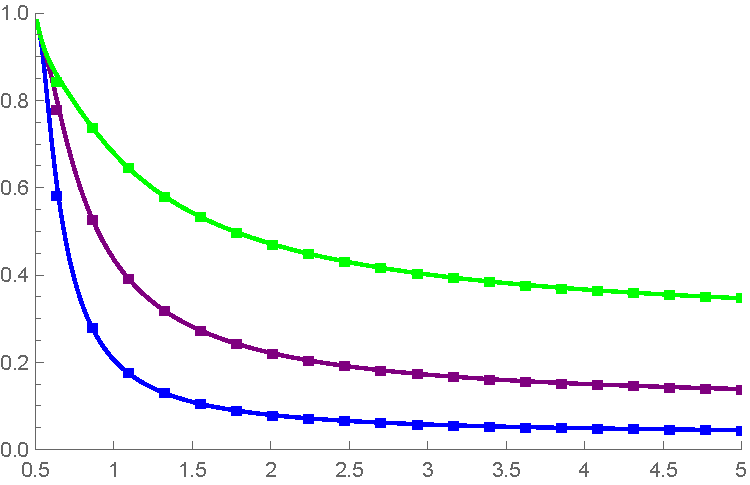
\includegraphics[scale=0.6]{figures/cn10000nu0512rep100a05to5Squares.pdf}
    \caption{Plot of $\gamma$ for $\alpha$ varying from $0.5$ to $5$ on the horizontal axis and 
    for $\nu=\frac{1}{2}$ (blue), $\nu=1$ (purple), $\nu=2$ (green); simulations (squares in corresponding colour) with $n=10000$ and $100$ repetitions.\label{fig:gamma}}
\end{figure}

In the above expression for $\gamma$, a factor $\alpha-1$ occurs in the denominator of each term, but we will see that this
corresponds to a removable singularity. We have not been able to find a closed form expression in terms of known functions in the case when $\alpha=1$, but in Section~\ref{ssec:alphais1} we do provide an explicit expression involving integrals.


\subsubsection{The clustering function}

Our second result is on the clustering function for constant $k$.

\begin{theorem}\label{thm:local_clustering_hyperbolic}\label{thm:mainkfixed}
Let $\alpha > \frac{1}{2}$, $\nu > 0$ and $k\geq2$ be fixed. 
Writing $G_n := G(n;\alpha,\nu)$, we have

\[
	c(k;G_n) \xrightarrow[n\to\infty]{\Pee} \gamma(k),
\]
where $\gamma(k)$ is defined for $\alpha \ne 1$ as 
\begin{align*}
\gamma(k)  =&\frac{1}{8\alpha (\alpha-1)\Gamma^+(k-2\alpha,\xi)} \left( -\Gamma^+(k - 2 \alpha, \xi) - 2\frac{\alpha (\alpha - 1/2)^2 \xi^{2} \Gamma^+(k - 2 \alpha - 2, \xi)}{(\alpha - 1)} \right. \\ 
&\left.+ 8 \alpha (\alpha - 1/2) \xi \Gamma^+(k - 2 \alpha - 1,\xi) \right.\\ 
&\left.+ 4\xi^{4\alpha - 2} \Gamma^+(k - 6 \alpha + 2, 
      \xi) \left( \frac{2^{ - 4\alpha}(3 \alpha - 1)}{(\alpha - 1)} + (\alpha - 1/2) B^-(1/2; 1 + 2 \alpha, -2 + 2 \alpha) \right)  \right.\\ 
&\left.+ \xi^{k-2\alpha} \Gamma(2\alpha+1)e^{-\xi} U(2\alpha+1,1+k-2\alpha,\xi) \right. \\ 
&\left.- \xi^{4\alpha-2} \Gamma(2\alpha+1)\MeijerGnew{3}{0}{2}{3}{1,3-2\alpha}{3-4\alpha,-6\alpha+k+2,0}{\xi}  \right)
\end{align*}
and for $\alpha = 1$ as the $\alpha\to1$ limit of the above expression.
% \begin{align*}
% 	c_\infty(k) &= \frac{9 \eta^3}{2 k!} 	
% 		\Gamma^+(k-3,\eta)-\frac{\xi^4}{k!}\frac{7+\pi^2}{4}\Gamma^+(k-4,\eta)\\
% 	&\hspace{10pt}+ \frac{\eta^k}{2k!}\int_0^1 (1-4z+3z^2)\ln(1-z)z^{1-k}e^{-\eta/z}\dd z\\ 
% 	&\hspace{10pt}+ \frac{\eta^k}{k!}\int_0^1 z^{3-k} \Li_2(z) e^{-\eta/z} \dd z,
% \end{align*}
% with $\eta = 4\nu/\pi$ and $\Li_2(z) = \sum_{t = 1}^\infty z^t/t^2$, the dilogarithm function.
\end{theorem}

\noindent
A plot of $\gamma(k)$ can be found in Figure~\ref{fig:gammak}. %
%
%
\begin{figure}[h!]
    \centering
    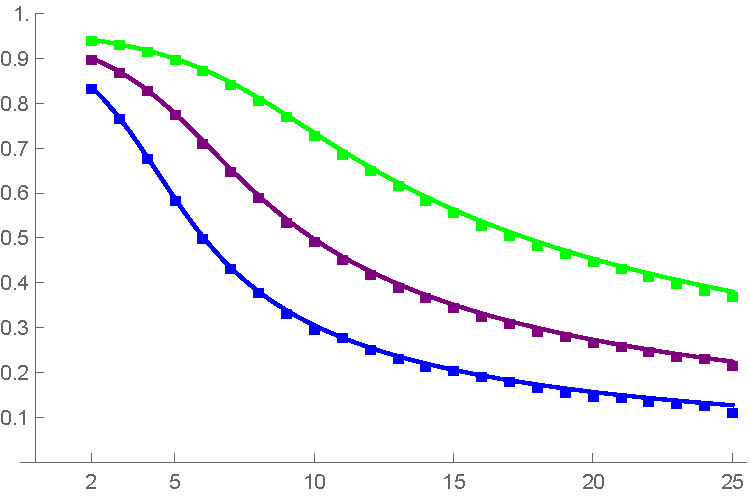
\includegraphics[scale=0.6]{figures/ckn10000a08nu0512rep100k2to25Squares.pdf}
    \caption{Plot $\gamma(k)$ for $k$ varying from 2 to 25 on the horizontal axis, for $\alpha=0.8$ and $\nu=\frac{1}{2}$ 
    (blue), $\nu=1$ (purple), $\nu=2$ (green); simulations (squares in corresponding colour) with $n=10000$ and $100$ repetitions.\label{fig:gammak}}
\end{figure}%
%
Again, we remark that the above expression for $\gamma(k)$ appears to have a singularity at $\alpha=1$, but this will turn out to be a removable singularity. Again, we have not been able to find a closed form expression in terms of known functions in the case when $\alpha=1$, but in Section~\ref{ssec:alphais1} we do provide an explicit expression involving integrals.

Theorem~\ref{thm:mainkfixed} in fact generalises to increasing sequences $(k_n)_n$.

\begin{theorem}\label{thm:mainktoinfty}
Let $\alpha>\frac12, \nu>0$ be fixed and let $k_n$ be a sequence of integers
satisfying $1 \ll k_n \ll n^{1/(2\alpha+1)}$. Then, writing $G_n := G(n;\alpha,\nu)$, we have
\[
	\E[|c(k_n;G_n)-\gamma(k_n)|] = \smallO{\gamma(k_n)},
\]
as $n \to \infty$, where $\gamma(\cdot)$ is as in Theorem~\ref{thm:mainkfixed}. In particular
\[
	\lim_{n \to \infty} \Exp{\left|\frac{c(k_n; G_n)}{\gamma(k_n)}- 1 \right|} = 0.
\]
\end{theorem}

%We remark that the number of vertices of degree exactly $k$ satisfies $N_k = 0$ a.a.s.~when $k \gg n^{1/(2\alpha+1)}$, see~\TM{ add reference to correct thm / lemma here! }.
%So the range in the above result is essentially to best possible.

\subsubsection{Scaling of $\gamma(k)$}

To clarify the scaling behaviour of $\gamma(k)$ with $k$ we offer the following result.

\begin{proposition}\label{prop:asymp}
As $k\to\infty$, we have

$$ \gamma(k) = 
(1+o(1)) \cdot \left\{ \begin{array}{cl}
\frac{8\alpha \nu}{\pi\left(4\alpha - 3\right)} \cdot k^{-1} &\text{ if } \alpha > \frac{3}{4}, \\
\frac{6 \nu}{\pi} \cdot \frac{\log(k)}{k}& \text{ if } \alpha = \frac{3}{4},\\
 c_{\alpha} \cdot k^{2-4\alpha} & \text{ if } \frac12 < \alpha < \frac34, 
\end{array} \right.,
$$
where $c_{\alpha} := \left( \frac{3\alpha - 1}{2^{4\alpha+1}\alpha(\alpha-1)^2} 
	+ \frac{(\alpha - \frac{1}{2})B^-(\frac{1}{2},2\alpha + 1, 2\alpha - 2)}{2(\alpha - 1)\alpha} 
	- \frac{B(2\alpha, 3\alpha - 4)}{4(\alpha - 1)} \right)  \cdot \xi^{4\alpha-2}$.
\end{proposition}

Note that Theorem~\ref{thm:mainktoinfty} implies that the clustering function of the KPKVB model scales as $\gamma(k)$ as $k$ grows, whose scaling is given in the above result. In particular, this contradicts the scaling conjectured in~\cite{krioukov2010hyperbolic} for $\alpha \leq \frac34$, and confirms it for $\alpha > \frac34$.

We remark that simultaneously and independently Stegehuis, van der Hofstad and van Leeuwaarden~\cite{stegehuis2018scale} found a similar, but less detailed result on the $k\to\infty$ scaling of the clustering function in the KPKVB model.

\subsection{Observations}

There are a few other observation to be made regarding our results.

\paragraph{Uniform convergence.}

Our results for the local clustering function in particular imply uniform convergence of $c(k; G_n)$ for all $2 \le k \le a_n$ where $a_n \ll n^{\frac{1}{2\alpha + 1}}$. To see this let
\[
	b_n = \arg \max_{2 \le k \le a_n} \Exp{\left|\frac{c(k_n; G_n)}{\gamma(k)} - 1\right|}.
\]
Then $b_n \le a_n \ll n^{\frac{1}{2\alpha + 1}}$ and therefore by Theorem~\ref{thm:local_clustering_hyperbolic}
\[
	\lim_{n \to \infty} \max_{2 \le k \le a_n} \Exp{\left|\frac{c(k; G_n)}{\gamma(k)} - 1\right|} 
	= \lim_{n \to \infty}\Exp{\left|\frac{c(b_n; G_n)}{\gamma(b_n)} - 1\right|} = 0.
\]


\paragraph{Near maximum scaling for $k_n$.}
Our results for the clustering function in the KPKVB model are valid for any sequence of integers $k_n \to \infty$ such that $k_n \ll n^{\frac{1}{2\alpha + 1}}$. Although one would like to have results for any sequence $k_n \le n$, it turns out that $n^{1/(2\alpha + 1)}$ is the near maximum scaling for which Theorem~\ref{thm:clustering_coefficient_hyperbolic} can be true. To see why this is the case note that by definition of the local clustering function~\eqref{eq:def_clustering_function} we have that $c(k_n; G_n) = 0$ if $N_{n}(k_n) = 0$, where $N_n(k_n)$ denote the number of vertices in a KPKVB graph $G(n; \alpha, \nu)$ with degree $k_n$. It follows by Markov's inequality that for any positive function $f : \R_+ \to \R_+$
\begin{align*}
	\Exp{\left|\frac{c_{\H,n}(k_n)}{f(k_n)} - 1\right|} 
	&\ge \Exp{\left|\frac{c_{\H,n}(k_n)}{f(k_n)} - 1\right|\ind{N_n(k_n) = 0}}\\ 
	&\ge \Prob{N_{n}(k_n) = 0} \ge 1 - \Exp{N_{\H,n}(k_n)}.
\end{align*}
We shall later establish (see Lemma~\ref{lem:diff_Nk_hyperbolic_binomial_poisson}) that $\Exp{N_n(k_n)}$ scales as $n k_n^{-(2\alpha + 1)}$. Therefore if $k_n$ is such that $k_n^{-(2\alpha + 1)} n$ tends to zero as $n \to \infty$ we have that 
\[
	\lim_{n \to \infty} \Exp{N_{n}(k_n)} = 0
\]
and hence
\[
	\lim_{n \to \infty} \Exp{\left|\frac{c(k_n; G_n)}{f(k_n)} - 1\right|} 
	\ge \lim_{n \to \infty} 1 - \Exp{N_{n}(k_n)} = 1 \ne 0,
\]
for any positive function $f$. This implies that we cannot expect a result like that of Theorem~\ref{thm:mainktoinfty} to hold as soon as $k_n \gg n^{\frac{1}{2\alpha + 1}}$.

\paragraph{Transition in scaling at $\bm{\alpha = 3/4}$.}

\PvdH{We should try and add something here. Not necessarily needed for the submission to arXiv though.}

\subsection{Outline of the paper}


In the next section we will recall some useful tools from the literature and define a series of auxiliary random graph models that will be used in the proofs. In particular, we relate in a series of steps the KPKVB model to an infinite percolation model $\Ginf$ that was used in previous work of the first and third authors~\cite{fountoulakis2018law} on the largest component of the KPKVB model. The value of the limiting constant $\gamma$, respectively limiting clustering function $\gamma(k)$, correspond to the probability that two randomly chosen neighbours of a ``typical point'' in this infinite model are themselves neighbours, respectively the probability of this event conditional on the typical point having exactly $k$ neighbours. These probabilities can be expressed as certain integrals, which we solve explicitly in Section~\ref{sec:Ginf}. 
In the same section we also prove Proposition~\ref{prop:asymp}, on the asymptotics of $\gamma(k)$. We then proceed to prove Theorems~\ref{thm:maincc} and~\ref{thm:mainkfixed} by relating said probabilities for the typical point of the infinite model to the corresponding clustering coefficient/function in the original KPKVB random graph, using the Campbell-Mecke formula and some other, relatively straightforward considerations.

The remaining sections are devoted to the proof of Theorem~\ref{thm:mainktoinfty}, which turns out to be a lot more involved. The main reason for this is that we push the possible scaling of $k_n$ to its maximum and hence a great deal of work is needed to properly control the arising error terms and make sure these are of smaller order than $\gamma(k_n)$. 

Finally, the Appendix includes some technical results on Meijer's G-function, Chernoff bounds for Poisson and Binomial random variables and the code used for simulations.

